\chapter{IRK: Eguzki-sistema.}

\section{Sarrera.}

Koordenatu kartesiarrak erabiltzearen abantaila.

\section{Eguzki-sistemaren integraziorako metodoak (review).}

\subsection{Efemerideak.}

Konputagailuen aurreko garaian, efemerideak teoria analitikoetan oinarritutako serie funtzioen bidez kalkulatzen ziren. Soluzio hauetan, Fourier serie trigonometriko luzeen ebaluazioa egin behar zen. $1960$ urteetan eguzki-sistemaren ezagutza hobetu zenean (accuracy of new observation types and space missions), serie oso luzeak kalkulatu behar zituzten, eta zenbakizko integrazioen bidezko soluzioak eraginkorragoak bilakatu ziren \cite{Kaplan2015}.   
   
Eguzki-sistemaren gorputzen efemeride modernoak, mugimenduaren ekuazio diferentzialen zenbakizko integrazioaren bidez kalkulatzen dira. Integrazioaren hasierako balioak eta ereduaren parametroak, sateliteen bidez jasotako datuei egokitzen zaizkie. 

Efemerideetarako eguzki-sistemaren eredu konplexua erabiltzen da. N-gorputz nagusien arteko indar grabitazionalez gain, erlatibitate efektua, asteroideek eragindako grabitazio indarrak, gorputzen formen eragina eta beste hainbat indar ez grabitazionalak kontutan hartzen dira. Mugimenduaren ekuazio diferentzialak  (Einstein-Imfeld-Hoffmann, $c^{-4}$ PPN hurbilketa) hauek dira,      
      \begin{equation*}
      \ddot{x}_{Planet}= \sum_{A \neq B} \mu_B \frac{r_{AB}}{\|r_{AB}\|^3}+\ddot{x}_{GR} (\beta,\gamma,c^{-4})+ \ddot{x}_{AST,300}+ \ddot{x}_{J_2}
      \end{equation*}
      
      \begin{itemize}
      \item $8$ planetak, Ilargia, Pluto eta 300 asteroide.
      \item GR: erlatibitate efektua.
      \item $J_2$: eguzkia esferikoa ez izatearen eragina. 
      \item Urrats luzeera, $h=0.055$ egunekoa da.
      \end{itemize}   

\paragraph*{Ekuazio diferentzialak (erlatibitate efektua).}
Eguzkiaren erlatibitate efektua kontutan hartzen duten ekuazio diferentzialak azalduko ditugu.

\begin{equation}
\dot{q_i}=v_i, \  i=0,1,\dots N
\end{equation}

\begin{multline} 
\dot{v_i}= \sum_{j=0,j \neq i}^{N} \frac{Gm_j}{\|q_j-q_i\|^3} (q_j-q_i)
           \bigg(1- \frac{2(\beta+\gamma)}{c^2} \sum\limits_{k=0, k \neq i}^{N} \frac{Gm_k}{\|q_k-q_i\|} 
                  - \frac{2\beta-1}{c^2}        \sum\limits_{k=0, k \neq j}^{N} \frac{Gm_k}{\|q_k-q_j\|} \\
                  + \gamma \big(\frac{v_i}{c}\big)^2 + (1+\gamma) \big(\frac{v_j}{c} \big)^2 
                  - \frac{2(1+\gamma)}{c^2} v_i \ v_j \\
                  - \frac{3}{2c^2} \big(\frac{(q_i-q_j) v_j}{\|q_j-q_i\|} \big)^2+                  
                  \frac{1}{2c^2}(q_j-q_i) \dot{v_i} \bigg) \\
           + \frac{1}{c^2} \sum_{j=0,j \neq i}^{N} \frac{Gm_j}{\|q_j-q_i\|^3} 
             ((q_i-q_l) ((2+2\gamma)v_i-(1+2\gamma)v_j)) (v_i-v_j) \\
           + \frac{3+4\gamma}{2c^2} \sum_{j=0,j \neq i}^{N} \frac{Gm_j \dot{v_j}}{\|q_j-q_i\|}                                      
\end{multline}

\begin{table}[h]
\caption{Konstanteak}
\label{tab:1}       % Give a unique label
\centering
\begin{tabular}{ c c c }
\hline
  c             &  $299792.458$ km/s           & Argiaren abiadura  \\
\hline
  au            &  $149597870.700$ km           & Astronomical unit  \\
\hline 	       
$\beta$          & $1.0$                       & PPN parametroa     \\
\hline 
$\gamma$         & $1.0$                       & PPN parametroa     \\
\hline
\end{tabular}
\end{table}

Asteroideek, bereziki Marte planetaren mugimenduarengan eragina dute eta kontutan hartzekoak, barne planeten mugimenduaren doitasun handiko emaitzak behar ditugunean. Bost asteroide nagusiren masak (Ceres, Pallas, Vesta, Iris eta Bamberga) Merkurio eta Pluto planeten mailakoak direnez, integrazioetan gehitzen dira. Beste asteroide txikien talde handia, estimazioen bidez simulatzen dira.

\begin{figure} [h]
\centerline{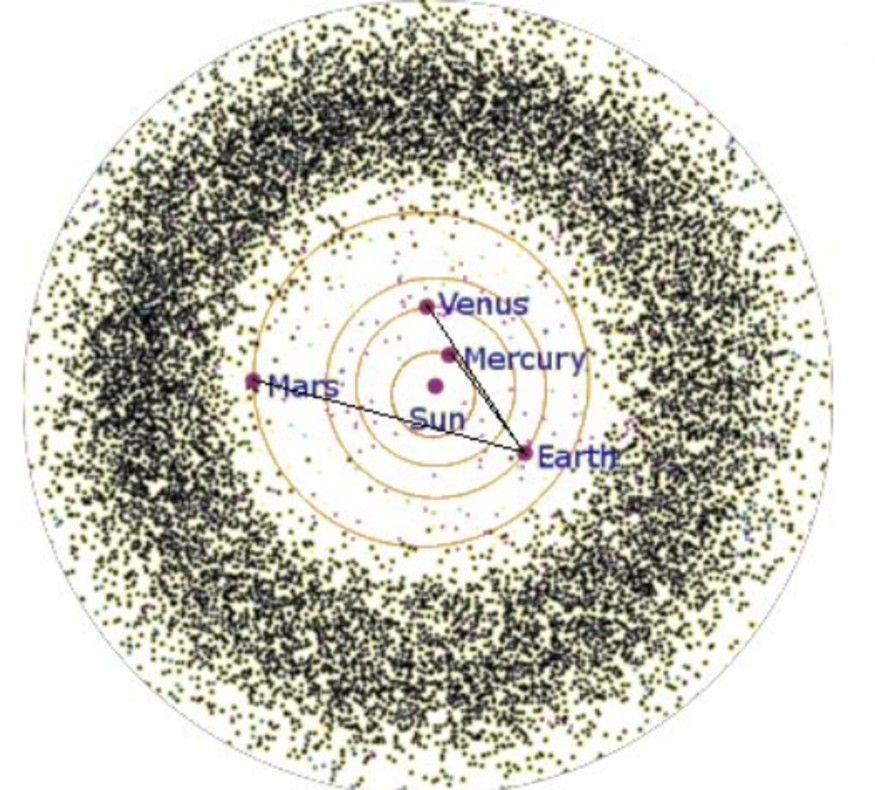
\includegraphics [width=8cm, height=6cm] {Asteroideak}}
\caption{Asteroideak.}
\label{fig:661}
\end{figure} 

Efemerideak \emph{Chebyshev} polinomio moduan adierazten dira. Integrazio tarteak, $2.000.$ urte inguruko ehunka urtekoak izaten dira. Zenbakizko integrazio hauetan, biribiltze errorea gai garrantzitsua da. $128$-biteko aritmetika erabiltzeko aukera oso garestia delako bere erabilera baztertzen da eta $64$-bit doitasuneko aritmetika hobetzeko teknika konputazionalki merkeak aplikatzen dira.
  
\paragraph*{}Hiru dira planetak efemerideak,
\begin{enumerate}
\item Jet Propulsion Laboratory (\emph{EEBB}) \emph{NASA}-ko erakundeak DE (Development Ephemerides) izeneko efemerideak.

      $1984$. urtean kalkulatu zen lehen efemeridea (DE-200) eta $2.014$. urteko da \emph{DE-430} \cite{Folkner2014} publikatutako azken efemeridea. Kalkulatutako integrazio tartea, ($1550-2650$) izan da.

      Zenbakizko integrazio metodoa. Urrats luzera eta  ordena aldakorreko \emph{Multistep Adams} metodoa, \emph{DIVA}/\emph{QIVA} (Krogh,1997). \emph{QIVA} doitasun laukoitzeko ($128$-bit) bertsioari deitzen zaio: mugimenduaren ekuazioen Newton zatia, doitasun laukoitzean kalkulatzen da eta ekuazioaren gainontzeko zatia, doitasun bikoitzean.

\item Institut de Méchanique Céleste et de Calcul des Ephémérides (IMCCE,Paris Observatory) INPOP (Intégrateur Númerique Planétaire de l'Observatoire de Paris) izeneko efemerideak.
      
      $2.000$. arte, teori analitikoetan oinarritutako efemerideak garatu zituzten. $2.003$. urtean kalkulatu zuten lehen zenbakizko integrazio bidezko efemeridea eta \emph{INPOP13c} ($2.014$) publikatutako azkena da.
           
	  Zenbakizko integrazio metodoa. Urrats finkoa eta $12$ ordeneko \emph{Adams-Cowell} metodoa da.
	  
	  Doitasuna. C lengoaian inplementatuta dago eta \emph{Intel} makinetako $80$-biteko doitasuna erabiltzen du. Era berean, modu merkean doitasun handitzeko, doitasun laukoitza simulatuz urrats zuzentzaile (corrector step) bat aplikatzen zaio \cite{Fienga2008}.  
	  
  
\item Institute of Applied Astronomy (\emph{IAA}, St. Petersburg), EPM (Ephemerides Planets-Moon) izeneko efemerideak.
      
      $1.980$. urtetik aurrera, zenbakizko integrazioen bidezko efemerideak kalkulatu dituzte eta  \emph{EPM2.013} ($2.014$) \cite{Pitjeva2014} publikatutako azken efemeridea da.
      
      Zenbakizko integrazio metodoa. \emph{Everhart} izeneko \emph{IRK} metodoa (Gauss-Radau) da. $23$ ordeneko metodoa eta urrats luzera finkoa erabiltzen du.
            
      Doitasuna. Inplementazioak (software package ERA), \emph{Intel} makinetako $80$-biteko doitasuna erabiltzen du.
      
\end{enumerate}


(\ref{fig:668}) taulan, planeten efemerideen doitasunaren eboluzioa ikus daiteke. Hiru efemerideak antzeko doitasuna azaltzen dutela aipatu beharra dago. 
\begin{figure} [h]
\centerline{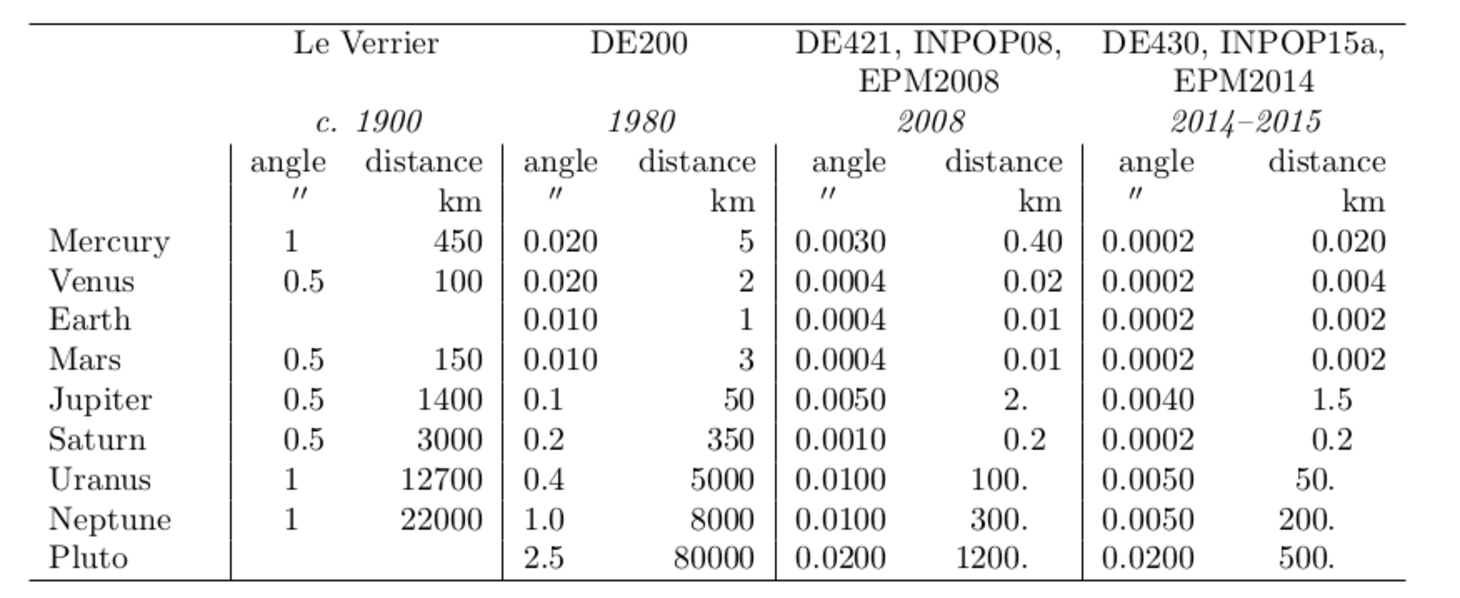
\includegraphics [width=10cm, height=6cm] {Efemerideak}}
\caption{Efemerideen doitasunaren eboluzioa.}
\label{fig:668}
\end{figure} 

\subsection{Eguzki-sistemaren integrazio luzeak.}


A.Morbidellik \cite{Morbidelli2002} eguzki-sistemaren zenbakizko integrazioen algoritmoen garapenaren azterketan, garai hauek bereizten ditu:

\begin{enumerate}

\item Garai klasikoa (The classical period).

$90$. hamarkada hasiera arte, urrats luzera aldakorreko integratzaileak erabiltzen dira: Runge-Kutta (Dormand et al. $1987$), Bulirsch and Stoer ($1966$), Radau (Everharht, $1985$), eta Störmer ($1990$). Garai honetan integrazio tarteak $10^4-10^6$ dira.  

\item Garai sinplektikoa (The symplectic period).

Wisdom eta Holmanen \ycite[1991]{Sussman1992} lanarekin, eguzki-sistemaren azterketarako integratzaile sinpletikoen erabilera zabaldu zen. Garai honetan, ($10^8-10^9$) integrazio tarteko eguzki-sistemaren azterketak egin ziren.  

\item Garai estatistikoa (The statistic period).

Planeten eta gorputz txikiren (asteroide, meteoritoak) arteko kolisio gertuko egoerak kalkulatzen dituzten algoritmoak garatu ziren. Inplementazio berri hauetan, milaka gorputzen integrazio azkarra egin daiteke. Horrela, asteroide eta meteoritoen orbiten distribuzio azterketa estatistikoak egin ziren.

\item Planeten sorrera azterketen garaia (The planetary accretion period).

Masa handiko gorputzen arteko kolisio gertuko egoerak kalkulatu daitezke eta beraz, eguzki-sistemaren sorrerari buruzko simulazioak nagusituko dira. 
 
\end{enumerate}

Mekanika zelestean bi integratzaile famili agertzen dira nagusi: integratzaile simetrikoak eta sinplektikoak. Metodo simetrikoetan urrats luzera tamaina aldakorreko integratzaileak, modu errezean inplementatu daitezke. Metodo simetrikoen artean nagusiena, 4 ordeneko \emph{Hermite} integratzailea (Aarseth \cite{Aarseth2008}) da. Hermite integratzailea konputazionalki garestia da eta bereziki, gorputz kopuru handia dituzten eta kolisio gertuko egoerak maiz gertatzen diren problemetan (eguzki-sistemaren sorrera, stellar dynamics, \dots) aplikatzen da.    
 
Gure lan eremua, eguzki-sistemaren epe luzeko integrazioak dira eta gaur-egun arlo honetan, nagusi bilakatu diren integratzaile sinplektikoak aztertuko  ditugu. Eguzki-sistemaren integrazio luzeei buruzko beste errebizio dokumentu interesgarri hauek aholkatu nahiko genituzke: \cite{Kholshevnikov2007} (Kholshevnikov2007, $2.007$), \cite{Brumberg2013} (Brumberg, $2.013$) eta  \cite{Ito2007} (Ito eta Tanikawa, $2.007$).

\subsubsection*{Eguzki-sistemari egokitutako integratzaile sinplektikoak.}

Wisdomek eta Holmanenek bere lanean \ycite[1991]{Sussman1992}, eguzki-sistemaren epe luzeko simulazioetarako integratzaile  sinplektikoak (\emph{WH}) arrakasta izan zuen. Eguzki sistema, mugimendu perturbatua duen sistema dinamikoa da eta ezaugarri honi egokitutako integratzaile eraginkorra garatu zuten. Metodoan n-planeten Hamiltondarra Jacobi koordenatuak  erabiliz, bi zatitan banatu zuten
\begin{equation*}
H(q,p)=H_K(p)+H_I(q) \ \ \ \mbox{non} \ \ \ H_K\gg H_I,
\end{equation*}
$H_K$, Hamiltondar Kepleriarra (planeten eguzkiarekiko mugimendu kleperiarra) eta $H_I$, Interakzioen Hamiltondarra (planeten arteko grabitazio interakzioak). Integrazioaren urrats bakoitzean , Hamiltondar bakoitzaren soluzioa tartekatuz, problema osoaren ebazpena kalkulatzen da.  

\emph{WH} integratzailea, ondorengo metodoen aurrekaria kontsideratu bada ere, bere aplikagarritasuna mugatua da. Batetik, izar anitzeko planeten sistemak edo planeta-ilargiak sistemak integratzeko ez da egokia. Bestetik, \emph{WH} metodo  sinplektikoa denez urrats luzera finkoarekin integratu beharra, eta hau, gorputzen arteko kolisio gertuko egoerak dituzten problemak modu eraginkorrean integratzeko eragozpen bat da. Arazo hauek gainditzeko, urteetan zehar algoritmo honen aldaerak proposatu dira eta jarraian, nagusienak aipatuko ditugu. 

Levinson eta Duncan-ek \ycite[1994]{Levison1994}, \emph{WH} inplementazioa, integratzaile ez sinplektiko batekin konbinatu zuten kolisio egoeren kalkulua hobetzeko. \emph{SWIFT} paketean \emph{RMVS3} izeneko integratzailea inplementatu zuten. Duncan, Levinson eta Lee-k \ycite[1998]{Duncan1998}, koordenatu Heliozentrikoak erabiliz, Hamiltondarra beste modu batean banatu zuten,  
\begin{equation*}
H(q,p)=H_K(p)+H_C(p)+H_I(q)
\end{equation*}
eta kolisio egoerak gertatzen diren unean, urratsa luzera txikituz aurre egin zioten. Inplementazioa \emph{SYMBA} izenekoa da. Chambers-ek \cite{Chambers1999} koordenatu Heliozentrikoetan oinarritu zen eta kolisio egoeretan, beste integratzaile  (Bulirsch-Stoer metodoa) batera aldatuz kalkulatzen ditu. Inplementazio honi \emph{MERCURY} izena eman zion. Levinson eta Duncan-ek ($2000$), aurreko inplementazioaren arazo batzuk konponduz,\emph{modified SYMBA} izeneko garapen berria egin zuten.
Kvaerno eta Leimkuhler \cite{Kvaerno2000} eta beste autore batzuk ere, antzeko ideiak landu dituzte.

Wisdom eta Holmanek proposatutko Hamiltondarraren banaketa, \emph{leapfrog} metodoaren bidez integratzen da eta beraz, 2 ordeneko da. Orden altuagoko ($p>2$) metodoak definitzeko, koefiziente negatiboak erabili behar dira \cite{Yoshida1993} \cite{Laskar2001} eta ez dira interesgarriak, \emph{leapfrog} metodoa hauek baino eraginkorragoa baita. 

\textbf{Adibidea.}Yoshidaren 4 ordeneko metodoa. $\phi_h$ oinarrizko metodoa \emph{leapfrog} izanik, metodoaren konposaketari dagokion 4 ordeneko konposizio metodoa,
\begin{equation*}
\Psi_h=\phi_{\gamma_1 h} \circ \phi_{\gamma_0 h} \circ \phi_{\gamma_{1 h}}.
\end{equation*}  
non  $\gamma_0=-2^{1/3}/(2-2^{1/3})$ eta $\gamma_1=1/(2-2^{1/3})$.

\paragraph*{} Beranduago, McLachlan-ek \ycite[1995]{McLachlan1995}, Laskar-ek eta Robutel-ek \cite[2001]{Laskar2001} koefiziente negatiboen arazoa gainditu zuten eta orden altuko splitting eskemak aurkitu zituzten. Laskar-Nature: "The stepsize is $2.5 \times 10^{-2}$ years, unless the eccentricity of the planets increases beyond about $0.4$, in which case the step size is reduced to preserve numerical accuracy". Berriki, Blanes et al \ycite[2012]{Blanes2013} orden altuko splitting eskema berriak eta eraginkorrak aurkitu ditu. 

Hernandez eta Bertschinger-ek \ycite[2015]{Hernandez2015} N-body problema grabitazional eta kolisiodunetarako 2 ordeneko integratzaile sinplektiko berri bat proposatu dute. Hernandez eta Bertschinger-ek \ycite[2015]{Hernandez2015} koordenatu kartesiarretan oinarrituz, N-Body problema 2-gorputzen problemetan banatzen dute. Honako Hamiltondarraren banaketa proposatzen dute,
\begin{align*}
H=T+V, \\
H=T+ \sum_{i} \sum_{i>j} V_{ij}, \\
H=T+ \sum_{i} \sum_{i>j} (K_{ij}-T{ij})
\end{align*}

\section{Gure inplementazioa.}

\subsection*{Sarrera.}

Demagun honako Hamiltondar banagarria dugula,
\begin{equation*}
H(y)=H_A(y)+H_B(y), \ \  \mbox{non} \ \ H_A \gg H_B.
\end{equation*}

Eta beraz, dagokion hasierako problema orokorra,
\begin{equation*}
\dot{y}=J^{-1}\triangledown H(y)=f(y) , \ \ y(t_0)=y_0.
\end{equation*}

\paragraph*{}$\dot{y}=f(y)$ , eredu sinple $k(y)=J^{-1}\triangledown H_A(y)$ eta eredu konplexu $g(y)=J^{-1}\triangledown H_B(y)$ baten arteko batura gisa deskonposatu daiteke,
\begin{equation*}
\dot{y}=f(y)=k(y)+g(y).
\end{equation*} 
Eredu sinplea konputazionalki merkea da eta eredu konplexua aldiz, garestia. Banaketa honekin, zati konplexuaren ebaluazio kopuru  txikienarekin integratu nahi dugu, zenbakizko integrazio eraginkorra lortzeko.

\subsection*{Eguzki-sistemaren ekuazioak.}

N-gorputzen problemaren Hamiltondarra, alde Kepleriarra (eguzkiarekiko interakzioa) eta planeten interakzioen batura gisa bana daiteke,
\begin{equation*}
H(q,p)=H_k+H_I, \ \ H_k \gg H_I.
\end{equation*} 
Eguzkiari dagokion azpindizea $i=0$ kontsideratzen badugu, 
\begin{align*}
H_k(q,p) &=\frac{1}{2} \sum\limits_{i=0}^{N} \frac{p_i^2}{m_i}-  \sum\limits_{i=1}^{N} \frac{Gm_0 \ m_i}{\|q_i-q_0\|}, \\
H_I(q) &=\sum\limits_{1\leq i < j \leq N}^{N} \frac{G \ m_i m_j}{\|q_j-q_i\|}
\end{align*}

Banaketa honi dagokion ekuazio diferentzialak,  $f(y)=k(y)+g(y)$ modu honetan laburtuko ditugu. Honako notazioa erabiliz,
\begin{equation*}
\dot{y}=f(y)=
\left(\begin{array}{c}
  \dot{q} \\
  \dot{v} \\
\end{array}\right)=
\left(\begin{array}{c}
  f_q(y) \\
  f_v(y) \\
\end{array}\right)=
\left(\begin{array}{c}
  k_q(y) \\
  k_v(y) \\
\end{array}\right)+
\left(\begin{array}{c}
  g_q(y) \\
  g_v(y) \\
\end{array}\right)
\end{equation*}

\paragraph*{}Batetik, $\dot{q}=f_q(y)$ ekuazio diferentzialen deskonposaketa honakoa da,
\begin{align*}
\dot{q}&=f_q(y)=v, \\
\dot{q}&=f_q(y) \ \Rightarrow \ \ 
\left \{ \begin{array}{c}
  k_q(y) =v_i, \ \ i=0,\dots,N. \\[.25cm]
  g_q(y) =0,\ \ i=0,\dots,N.\\
\end{array} \right.  
\end{align*}

\paragraph*{}Bestetik, $\dot{v}=f_v$ ekuazio diferentzialen deskonposaketa honakoa da,
\begin{align*}
\dot{v} &=f_v(y)=\sum_{j=0,j \neq i}^{N} \frac{Gm_j}{\|q_j-q_i\|^3} (q_j-q_i), \\
\dot{v} &=f_v(y) \ \ \Rightarrow \ \ 
\left \{ \begin{array}{c}
          k_v(y)=\left \{ \begin{array}{c}
           \dot{v}_0 =\sum_{j=1}^{N} \frac{Gm_j}{\|q_j-q_0\|^3} (q_j-q_0). \\[.30cm]
           \dot{v}_i = \frac{Gm_0}{\|q_0-q_i\|^3} (q_0-q_i), \ \  i=1,\dots,N.\\[.30cm]
         \end{array} \right. \\[.30cm]  
          g_v(y)=\left \{ \begin{array}{c}
             \dot{v}_0=0. \\[.30cm]
             \dot{v}_i= \sum_{j=1,j \neq i}^{N} \frac{Gm_j}{\|q_j-q_i\|^3} (q_j-q_i), \ \  i=1,\dots,N.\\[.30cm]  
           \end{array} \right. \\ 
         \end{array} \right.  
\end{align*}


\subsection*{Meta-algoritmoa.}

IRK metodoaren formulazioa gogoratuz,

\begin{align*}
\label{eq:62b}
Y_{n,i}&=y_n+ \sum\limits_{j=1}^{s} \mu_{ij} L_{n,j},  \ \ L_{n,i}=hb_if(Y_{n,i}), \ \ i=1,\dots,s,\\
y_{n+1}&=y_n+\sum\limits_{i=1}^{s} L_{n,i},
\end{align*}

S-ataleko IRK metodoaren iterazio bakoitzean, $Y \in \mathbb{R}^{s \times d}$ ezezagunetako ekuazio-sistema askatu behar dugu: 

\begin{equation*}
Y_{i}-y_n- \sum\limits_{j=1}^{s} \mu_{ij} \ hb_j \bigg(k(Y_{j})+g(Y_{j})\bigg)=0, \ \ i=1,\dots,s.
\end{equation*}

Gure planteamenduan ekuazio-sistema Newton-sinplifikatuaren bidez askatuko dugu, baina jakobiarraren kalkulurik gabe. Lortzen dugun metodoa, jakobiarraren hurbilpena alde kepleriarra kontsideratzen duen ($J=k'(Y_i)$) Newton-sinplifikatuaren baliokidea da. 

\subsubsection*{Garapena.}

\paragraph*{}Ekuazio-sisteman Newton metodoa aplikatuz. Soluziotik gertu dagoen balio batetik abiatuta, ($Y_i^{[0]}$) eta $k=1,2,\dots$, 
\begin{equation*}
\triangle Y^{[k]}=-\frac{F(Y^{[k]})}{F'(Y^{[k]})},
\end{equation*}

\begin{equation*}
Y^{[k+1]}=Y^{[k]}+\triangle Y^{[k]}.
\end{equation*}

IRK metodoaren ekuazio-sistemari aplikatuz,

\begin{equation*}
\triangle Y_i^{[k]}=-\frac{\big(Y_{i}^{[k]}-y_n- \sum\limits_{j=1}^{s} \mu_{ij} \ hb_j                               \big(k(Y_{j}^{[k]})+g(Y_{j}^{[k]})\big)\big)}
                          {\big(1-\sum\limits_{j=1}^{s} \mu_{ij} \ hb_j \big(k'(Y_{j}^{[k]})+g'(Y_{j}^{[k]})\big)\big)}
\end{equation*}

Ekuazio laburtzeko $\delta_i^{[k]}$ aldagai laguntzailea erabiliz hau da askatu beharreko ekuazio,

\begin{equation}
\triangle Y_i^{[k]}=\sum\limits_{j=1}^{s} \mu_{ij} \ hb_j \big(k'(Y_{j}^{[k]})+g'(Y_{j}^{[k]})\big)\triangle Y_j^{[k]}+\delta_i^{[k]},
\end{equation}

non,
\begin{equation*}
\delta_i^{[k]}=-Y_{i}^{[k]}+y_n+ \sum\limits_{j=1}^{s} \mu_{ij} \ hb_j \big(k(Y_{j}^{[k]})+g(Y_{j}^{[k]})\big).
\end{equation*}

Lortutako espresioa garatuko dugu.

\begin{enumerate}
\item \textbf{Lehen hurbilpena.}

$g'(Y_{j}^{[k]}) << k'(Y_{j}^{[k]})$  eta $g'(Y_{j}^{[k]})<\triangle Y_{j}^{[k]}$ denez,
\begin{equation}
\triangle Y_i^{[k]} \approx \sum\limits_{j=1}^{s} \mu_{ij} \ hb_j \ k'(Y_{j}^{[k]}) \ \triangle Y_j^{[k]}+\delta_i^{[k]}
\end{equation}  

\item \textbf{Bigarren hurbilpena (Linealizazioa).}

\begin{equation*}
k(Y_{j}^{[k+1]})=k'(Y_{j}^{[k]}) (Y_{j}^{[k+1]}-Y_{j}^{[k]})+k(Y_{j}^{[k]})+O(\|\triangle Y_j^{[k]}\|^2)
\end{equation*}
\begin{equation*}
\triangle Y_j^{[k]}=Y_j^{[k+1]}-Y_j^{[k]}
\end{equation*}

Honako hurbilpena,
\begin{equation*}
k'(Y_j^{[k]}) \triangle Y_j{[k]} \approx k(Y_j^{[k]}+\triangle Y_j^{[k]})- k(Y_j^{[k]})
\end{equation*}

ordezkatuz eta garatuz,
\begin{equation*}
\triangle Y_i^{[k]}=\sum\limits_{j=1}^{s} \mu_{ij} \ hb_j \ k(Y_j^{[k]}+\triangle Y_j^{[k]})\ -\sum\limits_{j=1}^{s} \mu_{ij} \ hb_j \ k(Y_j^{[k]}) +\delta_i^{[k]},
\end{equation*}

\begin{equation}
\triangle Y_i^{[k]}=-Y_i^{[k]}+y_n+ \sum\limits_{j=1}^{s} \mu_{ij} \ hb_j \ k(Y_j^{[k]}+\triangle Y_j^{[k]})\  +\sum\limits_{j=1}^{s} \mu_{ij} \ hb_j \ g(Y_{j}^{[k]}).
\end{equation}

\item \textbf{Ekuazioak berridatiziz.}

$\triangle Y_i^{[k]}=Y_i^{[k+1]}-Y_i^{[k]}$ definizioa erabiliaz,

\begin{equation}
Y_i^{[k+1]}=y_n+ \sum\limits_{j=1}^{s} \mu_{ij} \ hb_j \ k(Y_j^{[k+1]})\  +\sum\limits_{j=1}^{s} \mu_{ij} \ hb_j \ g(Y_{j}^{[k]}).
\end{equation}
\end{enumerate}


\subsubsection*{Meta-Algoritmoa.}
IRK metodoa aplikatzeko meta algoritmoa planteatuko dugu.

\begin{algorithm}[H]
 \BlankLine
  $y_0=float(y(t_0))$\;
  $e_0=float(y(t_0)-y_0)$\;
  \BlankLine
  \For{$n\leftarrow 0$ \KwTo ($endstep-1$)}
  {
   \BlankLine
    Hasieratu  $Y_{n,i}^{[0]},W_{n,i}^{[0]} \ \ , \ \ i=1,\dots,s $\;  
    $k=1 $\;
    $K_{n,i}^{[k]}=k(Y_{n,i}^{[k-1]}) $\;
    Askatu $Y_{n,i}^{[k]}=y_{n}+ \left(\sum\limits_{j=1}^{s} \mu_{ij} \ hb_j \ K_{n,j}^{[k]} \right) \ + (e_{n}+ W_{n,i}^{[k-1]}) $\;
   \BlankLine
   \While{ (konbergentzia lortu)}
   {
    \BlankLine 
    $k=k+1$\;
    $W_{n,i}^{[k-1]}=\sum\limits_{j=1}^{s} \mu_{ij} \ hb_j \ g(Y_{n,j}^{[k-1]}) $\;  
    $K_{n,i}^{[k]}=k(Y_{n,i}^{[k-1]}) $\;
    Askatu $Y_{n,i}^{[k]}=y_{n}+ \left(\sum\limits_{j=1}^{s} \mu_{ij} \ hb_j \ K_{n,j}^{[k]} \right) \ + ( e_{n}+ W_{n,i}^{[k-1]}) $\;
   }
   \BlankLine
   \eIf{$(NormalizeDistance(Y^{[k]},Y^{[k-1]})>1$}
   {$exit$\;}
   {$F_{n,i}^{[k]}=f(Y_{n,i}^{[k]}) $\;
    $L_{n,i}^{[k]}=hb_i \ F_{n,i}^{[k]} $\;
    $(y_{n+1},e_{n+1})\leftarrow BaturaKonpensatua(y_n,e_n,L_n^{[k]},F_n^{[k]})$\;}    
   \BlankLine
   \BlankLine
 }
 \caption{Main Algorithm}
\end{algorithm}

\paragraph*{} Meta-algoritmoari buruzko hainbat ohar:

\begin{enumerate}
\item Barne iterazioak.

Barne iterazioan, metodo egokiena aplikatu daiteke. Problema ez-stiffa bada, puntu finkoaren bidez askatu daiteke eta problema stiffa bada Newton sinplifikatuaren bidez. 

\paragraph*{} Puntu finkoaren bidezko barne-iterazioa :

\begin{algorithm}[H]
 \BlankLine
  $l=0$\;
  $Y_{n,i}^{[k,0]}=Y_{n,i}^{[k-1]}$\;
  \While{ (konbergentzia lortu)}
  {
   \BlankLine
   $l=l+1$\;  
   \BlankLine
   $K_{n,i}^{[k,l]}=k(Y_{n,i}^{[k,l-1]})$\;
   $Y_{n,i}^{[k,l]}=y_{n} + \left(\sum\limits_{j=1}^{s} \mu_{ij} \ hb_j \ K_{n,j}^{[k,l]} \right) \ + (e_{n} + W_{n,i}^{[k-1]}) $\;
  }
 \caption{Main Algorithm}
\end{algorithm}


\item Problema independenteak.

Era honetako deskonposaketa bat dugunean,

\begin{align*}
f\left ( \begin{array}{c}
   y_1 \\
   y_2 \\
\end{array} \right)=
\left ( \begin{array}{c}
   k_1(y_1) \\
   k_2(y_2) \\
\end{array} \right)+
\left ( \begin{array}{c}
   g_1(y_1,y_2) \\
   g_2(y_1,y_2) \\
\end{array} \right),
\end{align*}

eredu sinplifikatua problema independenteak osatzen dituzte eta barne iterazioak modu independentean kalkula daitezke. N-gorputzen eguzki-sistemaren adibidean, eredu sinplifikatua $k(y)$ (eguzkiarekiko interakzioa) planeta bakoitzarentzat problema independentea dugu. Kasu honetan urrats bat finkatuta, kanpo planeten $k(y)$ problema barruko planeta baino azkarrago konbergituko du. 

\end{enumerate}


\subsubsection*{Orokorpena.}

Aurreko atalean, maila bakarreko ereduen deskonposaketa aztertu dugu. Ideia orokortuz, eredu deskonposaketa maila ezberdinetan egin daiteke. Problema bat emanda $\dot{y} =f(y)$, 

\begin{align}
\mbox{1. maila} \ \
\left \{ \begin{array}{c}
  \mbox{Eredu osoa.   } f(y) \\[.25cm]
  \mbox{Eredu sinplea.    } \tilde{f}(y)  \\
\end{array} \right.
\ \Rightarrow \ \
f =\tilde{f}+(f-\tilde{f})  
\end{align}

\begin{align}
\mbox{2. maila} \ \
\left \{ \begin{array}{c}
  \mbox{Eredu osoa.   }\tilde{f}(y) \\[.25cm]
  \mbox{Eredu sinplea.    }\tilde{\tilde{f}}(y)  \\
\end{array} \right.
\ \Rightarrow \ \
\tilde{f} =\tilde{\tilde{f}}+({\tilde{f}}-\tilde{\tilde{f}})  
\end{align}

\paragraph*{} \textbf{Adibidea.}

Demagun ekuazio diferentzialak, $m$ perturbazio funtzio dituela,
\begin{equation*}
\dot{y}=f(y)=k(y)+g_1(y)+g_2(y)+\cdots+g_m(y)
\end{equation*}
non $k(y)\ll g_k(y)$,  $k=1,\dots,m$.

\paragraph*{}$m=2$ deneko kasu partikulara aztertuko dugu,
\begin{equation*}
\dot{y}=f(y)=k(y)+g_1(y)+g_2(y).
\end{equation*} 

Askatu behar dugun ekuazio,
\begin{equation*}
\mbox{Askatu} Y_{n,i}=y_{n}+ \sum\limits_{j=1}^{s} \mu_{ij} \ hb_j \ (k(Y_{n,j})+g_1(Y_{n,j})+g_2(Y_{n,j})) 
\end{equation*}


\begin{algorithm}[H]
 \BlankLine
  $y_0=float(y(t_0))$\;
  $e_0=float(y(t_0)-y_0)$\;
  \BlankLine
  \For{$n\leftarrow 0$ \KwTo ($endstep-1$)}
  {
   \BlankLine
    Hasieratu  $Y_{n,i}^{[0]},W_{n,i}^{[0]} \ \ , \ \ i=1,\dots,s $\;  
    $k=1 $\;
    $K_{n,i}^{[k]}=k(Y_{n,i}^{[k-1]}) $\;
    Askatu $Y_{n,i}^{[k]}=y_{n}+ \left(\sum\limits_{j=1}^{s} \mu_{ij} \ hb_j \ K_{n,j}^{[k]} \right) \ + (e_{n}+ W_{n,i}^{[k-1]}) $\;
   \BlankLine
   \While{ (konbergentzia lortu)}
   {
    \BlankLine 
    $k=k+1$\;
    $W_{n,i}^{[k-1]}=\sum\limits_{j=1}^{s} \mu_{ij} \ hb_j \ g_2(Y_{n,j}^{[k-1]}) $\;  
    $K_{n,i}^{[k]}=k(Y_{n,i}^{[k-1]}) $\;
    Askatu $Y_{n,i}^{[k]}=y_{n}+ \left(\sum\limits_{j=1}^{s} \mu_{ij} \ hb_j \ K_{n,j}^{[k]} \right) \ + ( e_{n}+ W_{n,i}^{[k-1]}) $\;
   }
   \BlankLine
   \eIf{$(NormalizeDistance(Y^{[k]},Y^{[k-1]})>1$}
   {$exit$\;}
   {$F_{n,i}^{[k]}=f(Y_{n,i}^{[k]}) $\;
    $L_{n,i}^{[k]}=hb_i \ F_{n,i}^{[k]} $\;
    $(y_{n+1},e_{n+1})\leftarrow BaturaKonpensatua(y_n,e_n,L_n^{[k]},F_n^{[k]})$\;}    
   \BlankLine
   \BlankLine
 }
 \caption{Main Algorithm}
\end{algorithm}


\paragraph*{}Erlatibitate efektua gehitzerakoan, N-gorputzen problemari dagokion ekuazio diferentziala,

\begin{equation*}
\dot{y}=f(y), \ f(y)=k(y)+g(y)+rs(y)+rn(y),
\end{equation*}

\begin{lstlisting}
k(y): kepleriarra.
g(y): planeten arteko grabitazio interakzioak.
rs(y): eguzkiarekiko erlatibitate efektua.
rn(y): planeten arteko erlatibitate efektuak.
\end{lstlisting}

\subsubsection*{Adierazpena.}

Ekuazio diferentzialen deskonposaketak, zuhaitz moduan adieraz daitezke.

\begin{equation*}
\dot{y}=f(y).
\end{equation*}


\begin{tikzpicture}[scale=.8]
%\draw (-1,-2) grid (5,2);
\filldraw[black] (0,0) circle (2pt);
\end{tikzpicture}

\begin{equation*}
f\left ( \begin{array}{c}
   y_1 \\
   y_2 \\
\end{array} \right)=
\left ( \begin{array}{c}
   f_1(y_1) \\
   f_2(y_2) \\
\end{array} \right)+
\left ( \begin{array}{c}
   g(y) \\
\end{array} \right),
\end{equation*}

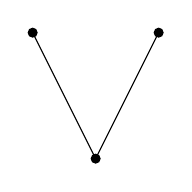
\begin{tikzpicture}[scale=.8]
%\draw (-1,-2) grid (5,2);
\filldraw[black] (0,0) circle (2pt);
\filldraw[black] (1,2) circle (2pt);
\filldraw[black] (-1,2) circle (2pt);
\draw (0,0) -- (1,2);
\draw (0,0) -- (-1,2);
\end{tikzpicture}

\begin{equation*}
f_1\left ( \begin{array}{c}
   y_1 \\
\end{array} \right)=
\left ( \begin{array}{c}
   f_{11}(y_{11}) \\
   f_{12}(y_{11},y_{12}) \\
   f_{13}(y_{11},y_{12},y_{13}) \\
\end{array} \right)+
\left ( \begin{array}{c}
   g_1(y_1) \\
\end{array} \right),
\end{equation*}


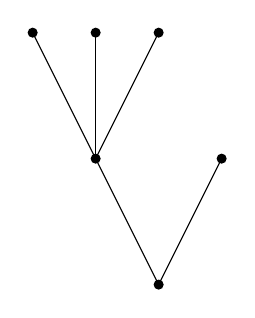
\begin{tikzpicture}[scale=.8]
%\draw (-1,-2) grid (5,2);
\filldraw[black] (0,0) circle (2pt);
\filldraw[black] (1,2) circle (2pt);
\filldraw[black] (-1,2) circle (2pt);
\filldraw[black] (-2,4) circle (2pt);
\filldraw[black] (-1,4) circle (2pt);
\filldraw[black] (0,4) circle (2pt);
\draw (0,0) -- (1,2);
\draw (0,0) -- (-1,2);
\draw (-1,2) -- (-2,4);
\draw (-1,2) -- (-1,4);
\draw (-1,2) -- (0,4);
\end{tikzpicture}


\section{Denbora birparametrizazioa.}

\subsection*{Sarrera.}

Uurrats luzera finkoa, ez da kolisio gertuko egoerak dituzten sistema dinamikoak edo denbora maila oso ezberdinak dituzten problemak integratzeko eraginkorra. Erregularizazio da arazo honen aurrean teknika arrakastatsuena. Erregularizazioaren bidez,  gorputzen arteko distantzia zerorantz hurbildu arren, mugimenduaren ekuazioak ez singularrak mantentzen dira.   

Demagun jatorrizko ekuazio diferentziala,
\begin{equation*}
\dot{y}=f(y(t)),
\end{equation*}

non $y$ menpeko aldagaia eta $t$ aldagai askea den.

\paragraph*{} Aldagai askeari aldaketa bat aplikatuz ($s()$ izeneko funtzio), ekuazio diferentziala leuntzea lortuko dugu. 

\begin{equation*}
y=z,
\end{equation*}

\begin{equation*}
\frac{dt}{d\tau}=s(z)
\end{equation*}

\paragraph*{} Honako garapena egingo dugu aldagai berriarekiko ($\tau$) ekuazioak lortzeko.

\begin{equation*}
y=z \ \ \Rightarrow \ \ \frac{dy}{dt}=\frac{dz}{d \tau} \ \frac{d \tau}{dt} \ \Rightarrow \ \frac{dz}{d \tau}= s(z) \ f(y(t)) 
\end{equation*}

\paragraph*{} Sistema berrian, mugimendua $z(\tau)$ funtzioak deskribatzen du: $z$ aldagai berria $\tau$ aldagai askearen menpekoa da. 

\subsection{Adibidea.}

Esperimentu honetan, IRK metodoan denbora birparametrizazioa modu errezean aplika daitekeela erakutsi nahi dugu. N9-Body probleman, merkurio ezentrizitate handiena duen planeta da: merkurio araberako denbora birparametrizazioa planteatuko dugu.

\begin{equation}
s(q)=r_{10}^{3/2}
\end{equation}

\begin{equation}
r_{10}=\|q1-q0\|_2
\end{equation}

non $q_1=(q1_{x},q1_{y},q1_{z})$ merkurio plantearen kokapena eta $q_0=(q0_{x},q0_{y},q0_{z})$ eguzkiaren kokapena den.

\section{Atalen hasieraketa.}

Eguzki sistemarako honako idei berri bat azalduko dugu. Honako ekuazio diferentziala dugularik,
\begin{equation*}
\dot{y}=k(y)+\epsilon \ g(y)
\end{equation*}

Alde kepleriarraren fluxua ezaguna dugu,
\begin{align*}
\varphi_{\triangle t}^k:&  \ \mathbb{R}^d \ \longrightarrow \mathbb{R}^d  \\
&  y_0 \longrightarrow y_1. 
\end{align*}

Aldagai aldaketa bat egin daiteke,
\begin{align*}
y(t_0+\triangle t) &= \varphi _{\triangle t}^k(z(t_0+\triangle t)), \ \ y(t_0)=z(t_0), \\
z(t_0+\triangle t) &= \varphi _{-\triangle t}^k(y(t_0+\triangle t)).
\end{align*}

Aldagai berriarekiko ekuazio diferentziala mantso aldatzen den funtzioa da,
\begin{align*}
\dot{z}=\epsilon \ r(z,t).
\end{align*} 

Ideia hau bi modutara aplika daiteke,
\begin{enumerate}
\item Gauss inplizituaren integrazio metodoan.
\item Atalen hasieraketa ona lortzeko.
Orokorrean, interpolazio bidezko hasieraketa ona izateko,  urratsa txikia izan behar du (periodo bat baino txikiagoa izan behar du). Teknika hau erabiliz, interpolazioaren errorea $\mathcal{O}(\epsilon)$ mailakoa izango da.

Proposamen honetan hasieraketa $z$ aldagai berria erabiliz era honetan egingo dugu:
\begin{itemize}
\item $Y_{n-1}$ atalei kepler \textbf{denboran atzeratuz}, $Z_{n-1}$ aldagai berriarekiko atalak lortuko ditugu.
\item $Z_{n-1}$ alatak interpolauz, $Z_{n}^{[0]}$ hasieraketak lortuko ditugu.
\item $Z_{n}^{[0]}$ atalei kepler \textbf{denboran aurreratuz}, $Y_{n}^{[0]}$ hasieraketak lortuko ditugu.
\end{itemize}


\end{enumerate}


\begin{figure}[!h]
\centering
\subfloat[Atalen hasieraketa1.]{
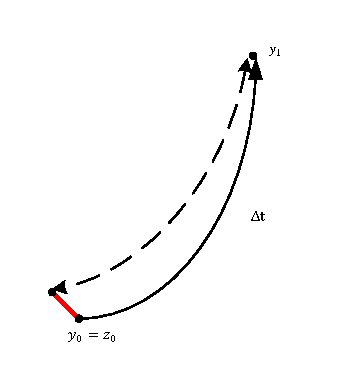
\includegraphics[width=.500\textwidth]{AtalenHasieraketa1}
}
\subfloat[Atalen hasieraketa2.]{
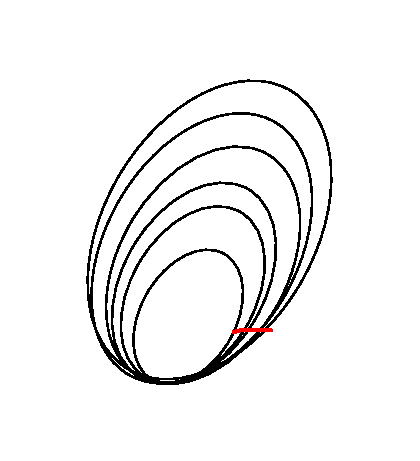
\includegraphics[width=.500\textwidth]{AtalenHasieraketa2}
}
\caption[Atalen hasieraketa.]
        {\small ....        
         \textbf{(a) irudian},                           
         \textbf{(b)} ......        
        }
\label{fig:Atalak12}
\end{figure}   

\begin{figure}[h]
\centerline{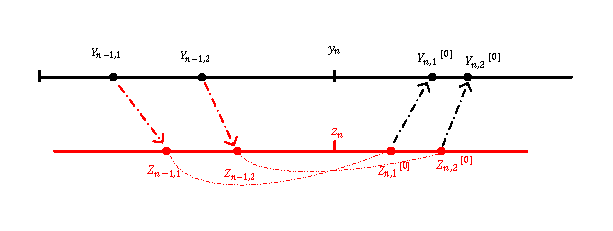
\includegraphics[width=12cm, height=6cm] {AtalenHasieraketa3}}
\caption{Atalen hasieraketa3.}
\label{fig:lau}
\end{figure} 

\section{Laburpena.}